%!TEX root = ./cikm2016.tex
\section{Knowledge Completion}
\label{sec:exp1}

\begin{table}[t]
\centering
\caption{\label{tbl:dataset}Description of datasets. 
Sparsity denotes the ration of valid triples to invalid triples.}
\vskip 0.15in
\begin{tabular}{l | r | r | r | r}
Dataset &  \# rel & \# entities & \# triples & sparsity \\ \hline
Kinship & 26 & 104  & 10,790 & 0.038 \\
UMLS & 49 &135  & 6,752 & 0.008 \\
Nation & 56 & 14  & 2,024 & 0.184 \\
%Wordnet & 11 & 38,696  &123,429 & 7.5e-06\\
%Wordnet(N) & 10 & 836 & 1,766 & 2.5e-04\\
\end{tabular}
\end{table}


\begin{figure}[t]
	\centering
	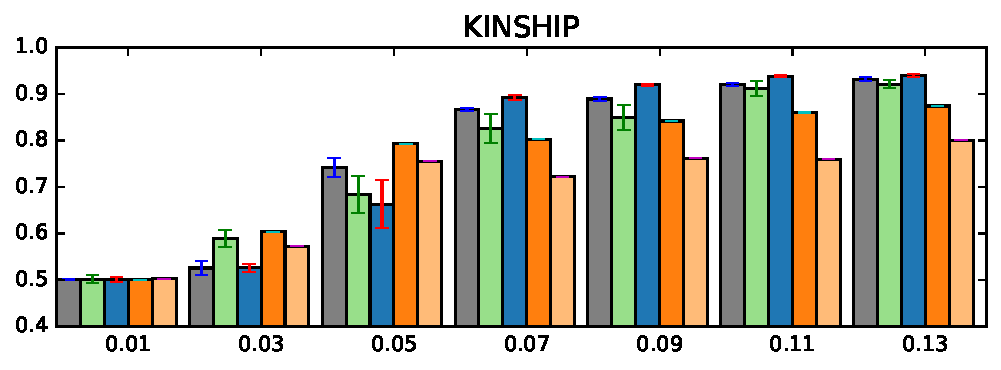
\includegraphics[width=\linewidth]{images/comp_training_error_kinship_small.pdf}
	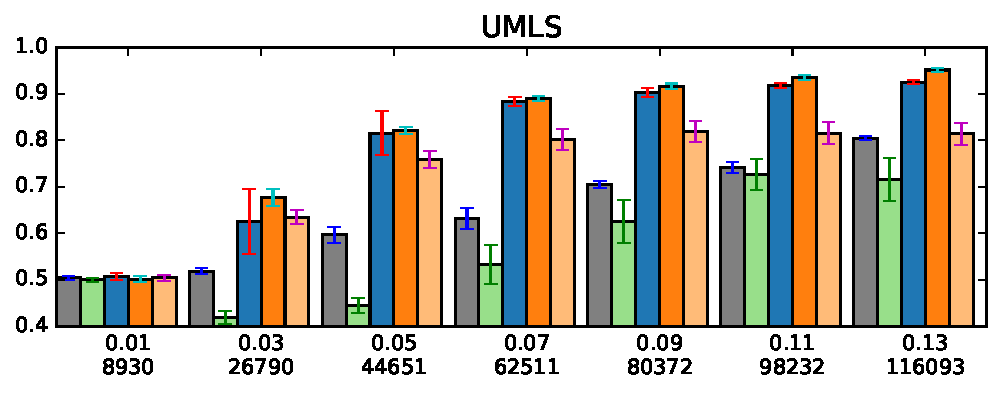
\includegraphics[width=\linewidth]{images/comp_training_error_umls_small.pdf}			
	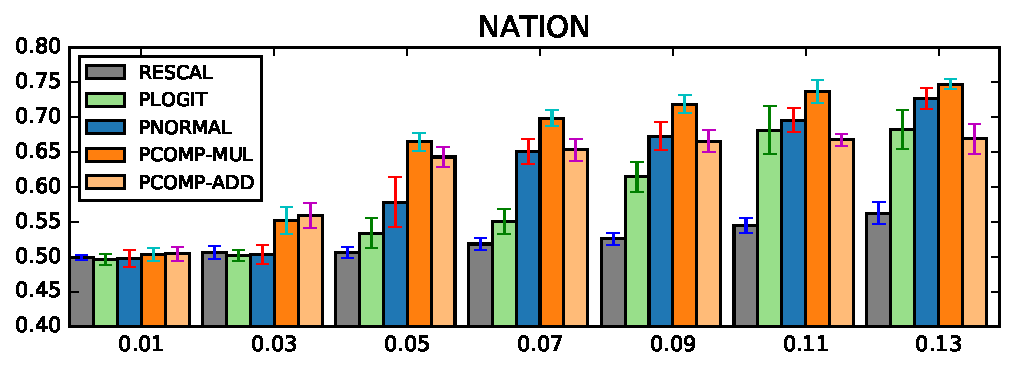
\includegraphics[width=\linewidth]{images/comp_training_error_nation_small.pdf}				
	\caption{\label{fig:r_vs_br} ROC-AUC scores of compositional models. 
	The x-axis denotes the proportion and total number of triples used for training. %We use other 20\% of triples as a validation set and another 30\% of triples as a test set. 
}
\end{figure} 

%Applying Thompson sampling to the compositional models is not straight forward. 
%Because, in the compositional model, adding one valid triple in a knowledge base will 
%change the accompanying compositional paths over the extended tensor $\mathcal{X}^L$. 
%Therefore, the system requires to compute potential changes in the 
%compositional structure for every candidate query triple. This computational complexity 
%will increase exponentially as we increase the length of the composition.

%In this experiment, instead running the Thompson sampling for the compositional models,
We first evaluate our model for the knowledge completion task
%we follow the standard train/validation/test approach 
to measure the performance of PRESCAL with all non compositional and compositional variants.
%The results between active acquisition and training and testing are not always coincident, but if the Thompson sampling samples latent features from true posterior of the compositional model, the samples corresponds to the true posterior samples from the training set.

We evaluate the PRESCAL models on three benchmark datasets and compare the performance to various baseline 
algorithms. We use three relational datasets: KINSHIP, UMLS, and NATION. Detailed description of each 
dataset is shown in Table \ref{tbl:dataset} \footnote{https://alchemy.cs.washington.edu/papers/kok07/}.


For all experiments, we set the compositional length $L$ to 2, split the dataset into 20\% for validation and 30\% for testing. We vary the proportion of training triples
from 1\% to 13\% of datasets. For RESCAL, we use the authors' implementation, and measure performance over 10 runs with random initialisations. For PRESCAL and all the variants, we sample triples $x_{ikj}$ from its posterior, and measure performance over 10 different samples.
%Based on the trained model, measure the ROC-AUC scores on the test set.
Given the test set, the performances of models are measured by ROC-AUC score:
\begin{align}
\frac{1}{|\mathcal{X}_p|  |\mathcal{X}_n|} \sum_{\{i,k,j\} \in \mathcal{X}_p, \{i',k',j'\} \in \mathcal{X}_n} \mathbb{I}[\bar{x}_{ikj} > \bar{x}_{ikj}],
\end{align}
where $X_p$ and $X_n$ are the set of positive and negative triples in the test set, respectively, and $\bar{x}$ is a reconstructed triple.

Figure \ref{fig:r_vs_br} shows the ROC-AUC scores of the compositional models with the various baseline models. We can see that the PRESCAL with the normal output (PNORMAL) or logistic output (PLOGIT) generally outperform RESCAL. We compare the compositional model with original RESCAL, PNORMAL, and PLOGIT. In general, the multiplicative compositional model (PCOMP-MUL) outperforms the additive compositional model (PCOMP-ADD), and performs better the other baseline models when the proportion of training set is small. For UMLS and NATION, BCOMP-MUL outperforms across the all training proportions. For KINSHIP, however, the model performs better when the training proportion is less than 7\%.

We visualise the multi-dimensional entities inferred from RESCAL and PNORMAL of the NATION dataset into the two-dimensional space through tSNE \cite{VanDerMaaten2008} in Figure \ref{fig:tsne}. The probabilistic interpretation gives a systematic way to measure the uncertainty of obtained entities while the RESCAL cannot.

\begin{figure*}[t]
	\centering
	
	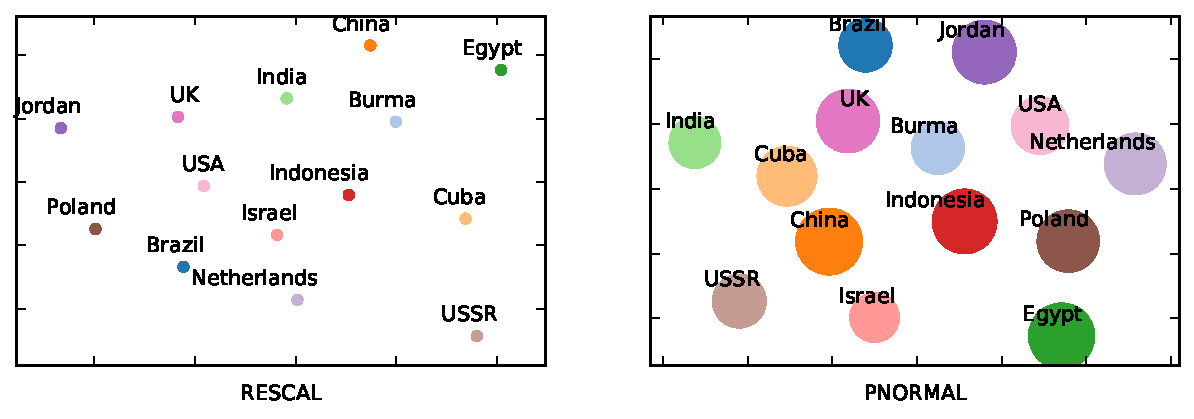
\includegraphics[width=0.8\linewidth]{images/embedding_nation.pdf}

	\caption{\label{fig:tsne} Embedding multi-dimensional entities of the NATION dataset into the two-dimensional space through tSNE \cite{VanDerMaaten2008}. The size of circle in PNORMAL is proportional to the uncertainty of entities in the embedded space. The probabilistic interpretation gives a systematic way to measure the uncertainty of obtained entities.}
\end{figure*}

\section{Active Knowledge Population}
\label{sec:exp2}

In this section, we show results for Thomson sampling of the PRESCAL and its compositional variants, first, on two synthetic datasets, and then on three common benchmarks used in the knowledge graph completion task.
%\rev{These experiments compare exploitation and exploration
% with exploitation only algorithms, and also show how the compositional model
%improves the entity embedding upon the non-compositional models. }
%%LX: second sentence can be cut if we need space.

\subsection{\rev{Thompson Sampling on }synthetic data}
\begin{figure}[t]
	\centering
	\subfigure[\scriptsize Logistic: N=10, K=10, D=5\label{fig:syn1}]{
	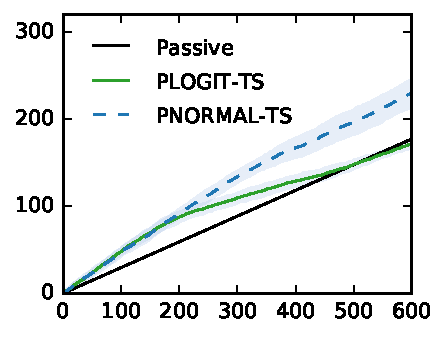
\includegraphics[width=0.42\linewidth]{images/toy_logit_vs_normal_10_10_5.pdf}
	}
	\subfigure[\scriptsize Logistic: N=20, K=10, D=5\label{fig:syn2}]{
	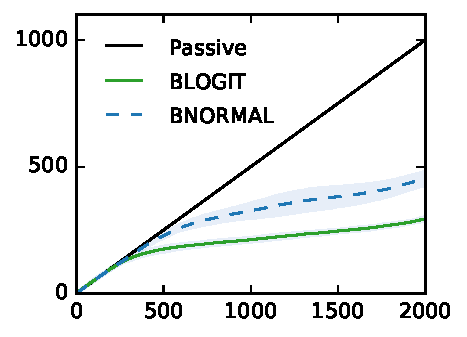
\includegraphics[width=0.445\linewidth]{images/toy_logit_vs_normal_20_10_5.pdf}
	}
	\subfigure[\scriptsize Gaussian: N=10, K=10, D=5\label{fig:syn3}]{
	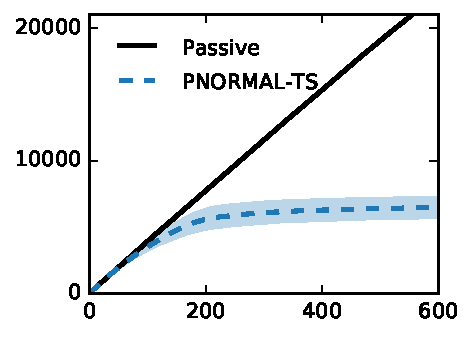
\includegraphics[width=0.42\linewidth]{images/toy_10_10_5.pdf}
	}
	\subfigure[\scriptsize Gaussian: N=20, K=10, D=5\label{fig:syn4}]{
	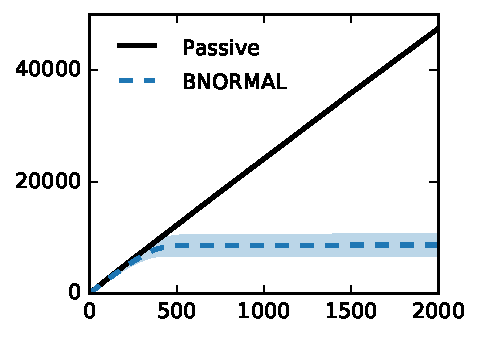
\includegraphics[width=0.45\linewidth]{images/toy_20_10_5.pdf}				
	}
%	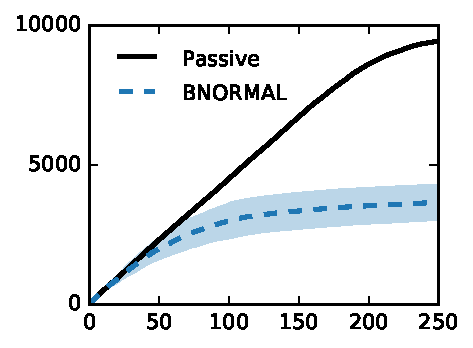
\includegraphics[width=0.32\linewidth]{images/toy_5_10_5.pdf}			
%	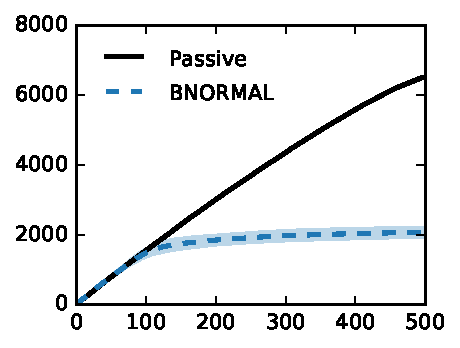
\includegraphics[width=0.32\linewidth]{images/toy_10_5_5.pdf}				
	\caption{\label{fig:synthetic} Cumulative regret of particle Thompson sampling with Gaussian and logistic output (PNORMAL-TS, PLOGIT-TS) against Passive learning 
	on synthetic datasets with logistic	(top row, a, b) and Gaussian (bottom row, c, d) output variables.
	%We compared the particle Thompson sampling with passive sampling method. 
	The averaged cumulative regrets over 10 runs are plotted with one standard error. 
	As the model obtained more and more labeled samples from Thompson sampling, 
	the cumulative regrets increase sub-linearly.}
\end{figure}

We first synthesise two datasets 
following the model assumptions in Eq. \ref{eqn:entity_gen} to 
\verify{\ref{eqn:triple_gen}}. 
\eat{We randomly generate triples based on randomly sampled entities and relations. Every }
\rev{First, }entities and relations are generated from zero-mean isotropic multivariate normal distribution, \eat{where we set }\rev{with } 
variance parameters $\sigma_e=1$, $\sigma_r=1$, respectively.
\rev{We generate two sets of \eat{the final}output triples,}
\eat{we generate two sets of datasets with }
\rev{with} the logistic output \eat{output variable }and the Gaussian \rev{with $\sigma_x$ set to 0.1}\eat{ variable}, respectively (Sec~\ref{sec:brescal}). 
\eat{The variance of gaussian $\sigma_x$ set to 0.1.}

To measure performance\eat{ on synthetic dataset}, we compute cumulative regret 
\eat{of proposed algorithm }at each time $n$ as $R(n) = \sum_{t=1}^{n} x_t - x^{*}_t$, 
%\begin{align}
%R(n) = \sum_{t=1}^{n} x_t - x^{*}_t,
%\end{align}
where $x^*_t$ is the highest\rev{-valued} triple among triples that have not been chosen up to time $t$. Unlike the general 
bandit setting where one can select a single item multiple times, in our formulation, we can select one triple 
only once. So after selecting a triple at time $t$, the selected triple will be removed from a set of candidate 
triples.

Figure \ref{fig:synthetic} shows the cumulative regret of the algorithm on the synthetic data with varying size of 
entities and relations. We compare the cumulative regret of the particle Thompson sampling with the passive 
learning method where the model choose a random triple at each time. All results are averaged over 10 
individual runs with different initialisations. 
Note that the dataset with binary logistic output variables can be used to train both logistic-output PRESCAL (PLOGIT) and Gaussian-output PRESCAL (PNORMAL) whereas the dataset with the Gaussian output can only be trained by PNORMAL.
Figure \ref{fig:syn1} and \ref{fig:syn2} show that with the logistic synthetic dataset both models are capable to learn the latent features of the generated triples, with logistic outperforming the Gaussian; Figure \ref{fig:syn3} and \ref{fig:syn4} show that the Thompson sampling for PNORMAL (PNORMAL-TS) \rev{outperform passive learning in} the real valued dataset. 
%For every experiment, the cumulative regret of the Thompson 
%sampling method was bounded after a certain number of interactions whereas the cumulative regret of 
%passive learning increases linearly. 
\eat{Both results indicate the particle sampling is capable of inferring latent features 
of entities and relations as the interaction increases.}

\subsection{Thompson sampling for compositional\\ models on synthetic data}
\begin{figure}[t]
	\centering
	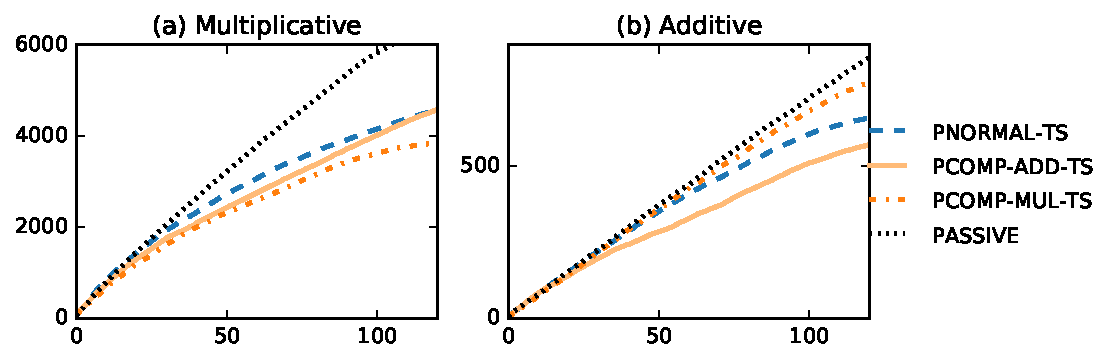
\includegraphics[width=\linewidth]{images/toy_comp_5_2_5.pdf}
	\caption{\label{fig:comp_synthetic} Cumulative regret of particle Thompson sampling of the compositional models on synthetic dataset with N=5, D=5. The synthetic dataset has three relations (K=3); the first two are independently generated, and the third relation is composed by the first two relations. The dataset used in (a) is generated by the multiplicative assumption, and the dataset used in (b) is generated by the additive assumption.}
\end{figure}

We conduct a second experiment on synthetic dataset to understand how
the Thompson sampling works for the compositional data. 
As in the first experiment, we first generate entities and relations from 
zero-mean multivariate normal with variance parameter $\sigma_e = 1$ and 
$\sigma_r=1$. We generate a set of triples with Gaussian output as in 
Eq. \ref{eqn:triple_gen}. We then synthesise two sets of expanded tensors 
using the previously used entities and relations based on the multiplicative 
and additive compositional assumptions, defined in Sec \ref{sec:comp}, 
respectively. So we synthesise fully observable expanded tensor $\mathcal{X}^L$ 
where $L=2$. We set both variance parameter $\sigma_x$ and $\sigma_c$ to 0.1. Note that in real world situation, the expanded tensor can be only constructed through the observed triples, and the triples in the expanded tensor cannot be queried.


\begin{figure*}[t]
	\centering
	
	\subfigure[KINSHIP]{
	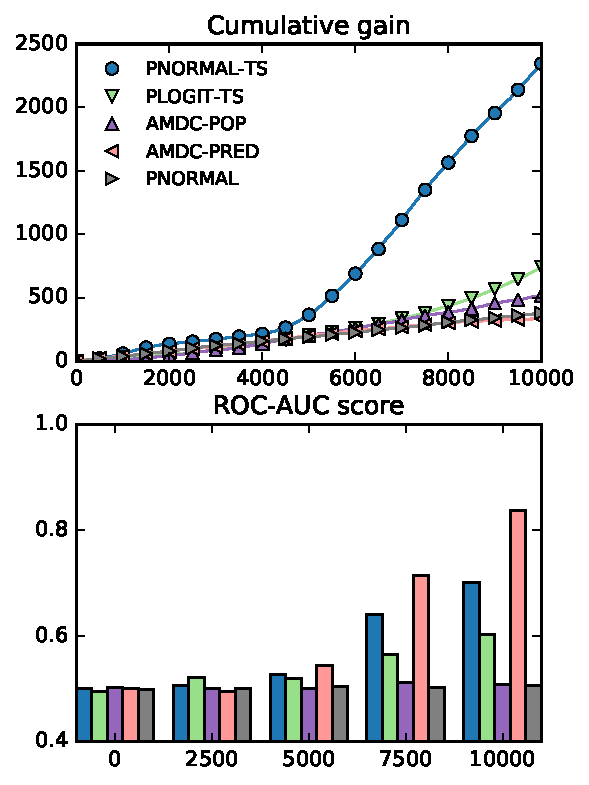
\includegraphics[width=0.3\linewidth]{images/present_vs_passive_greedy_thompson_kinship_mcmc_vertical_line.pdf}
	}
	\subfigure[UMLS]{
	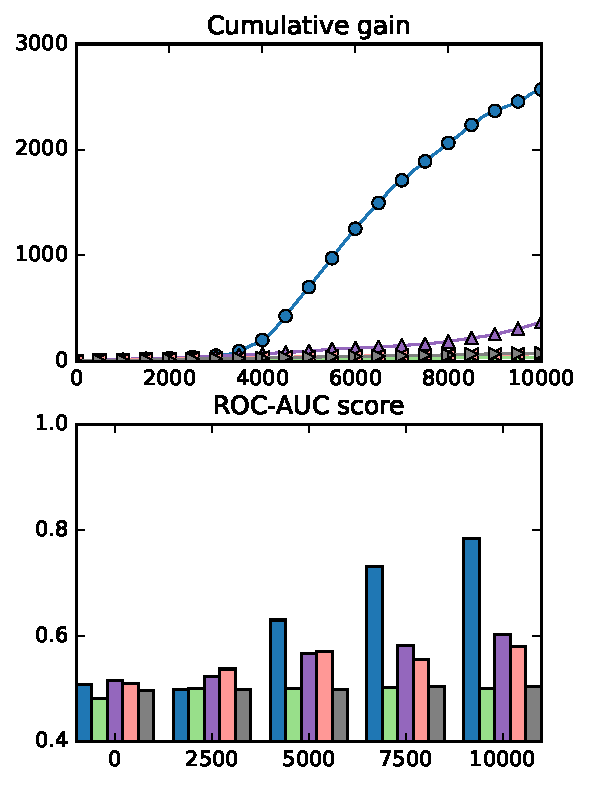
\includegraphics[width=0.3\linewidth]{images/present_vs_passive_greedy_thompson_umls_mcmc_vertical_line.pdf}				
	}
	\subfigure[NATION]{
	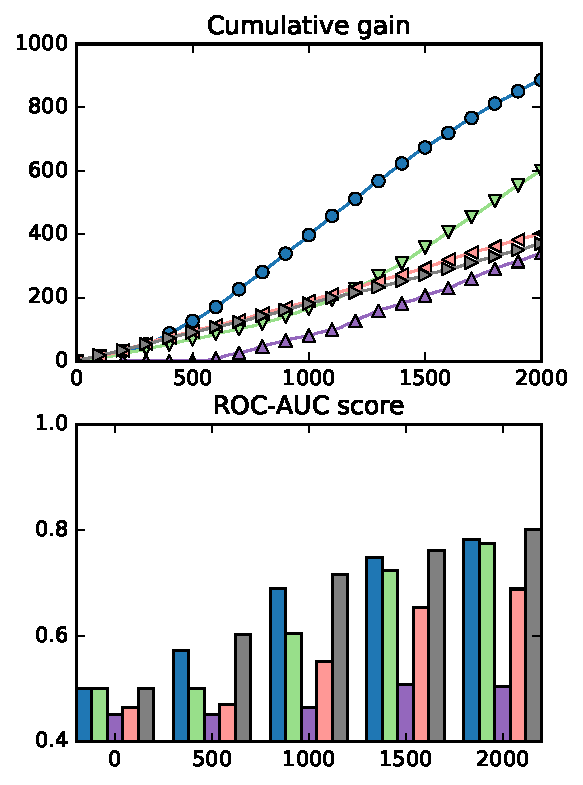
\includegraphics[width=0.3\linewidth]{images/present_vs_passive_greedy_thompson_nation_mcmc_vertical_line.pdf}				
	}	
	\caption{\label{fig:vs_greedy} The cumulative gain and ROC-AUC score of the Thompson sampling with passive learning and  AMDC models. Thompson sampling with PRESCAL (PNORMAL-TS) model achieves the highest cumulative gain to compare with AMDC and passive learning algorithms and shows comparable performance on ROC-AUC scores.}
\end{figure*}

\begin{figure*}[t]
	\centering
	
	\subfigure[KINSHIP]{
	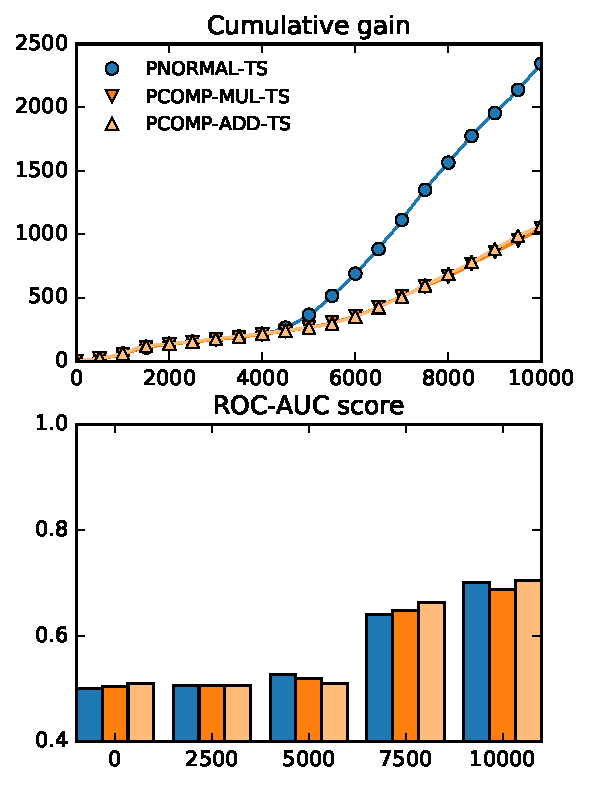
\includegraphics[width=0.3\linewidth]{images/present_vs_comp_thompson_kinship_mcmc_vertical_line.pdf}
	}
	\subfigure[UMLS]{
	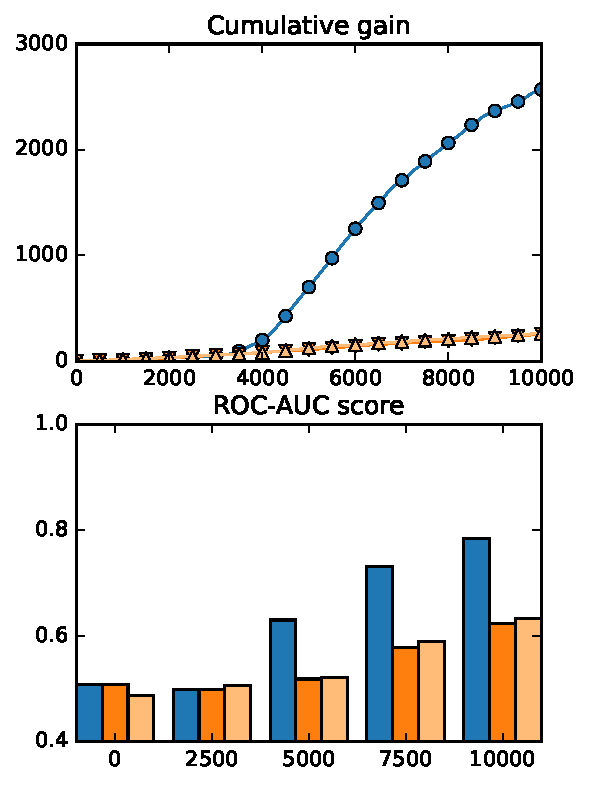
\includegraphics[width=0.3\linewidth]{images/present_vs_comp_thompson_umls_mcmc_vertical_line.pdf}				
	}
	\subfigure[NATION]{
	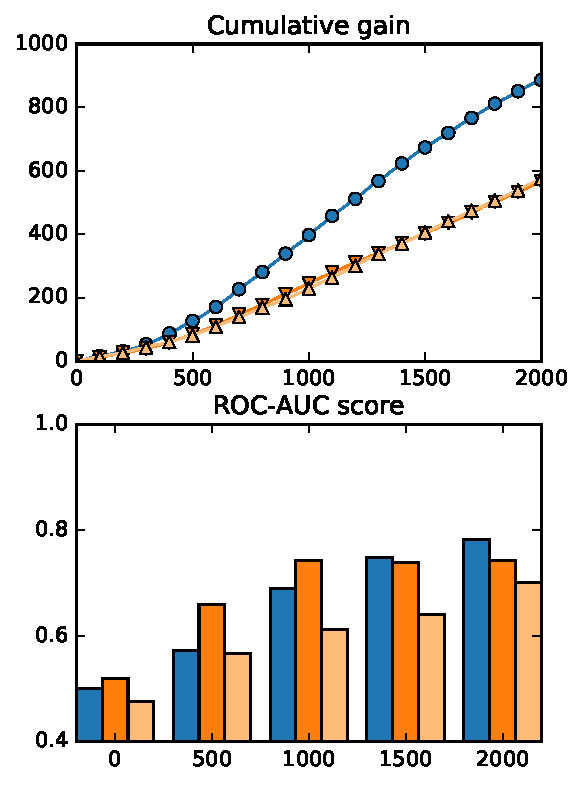
\includegraphics[width=0.3\linewidth]{images/present_vs_comp_thompson_nation_mcmc_vertical_line.pdf}				
	}	
	\caption{\label{fig:vs_comp} The cumulative gain and ROC-AUC score of the Thompson sampling with the non-compositional model and compositional models. Unlike the knowledge completion task in Section \ref{sec:exp1}, both compositional models perform worse than PNORMAL-TS in the active knowledge acquisition.}
\end{figure*}


To run the particle Thompson sampling on the synthetic dataset, we let the 
compositional models know which relation is composed by other relations. 
The non-compositional PNORMAL model assumes each relation is independent to one another. 
Therefore, the compositional model uses much less number of parameters to model 
the same size of tensor to compare with the non-compositional model. 
\eat{%%LX: these info repeats?
Through 
this experiments, we verify the particle Thompson sampling algorithm for the 
compositional models.

For the experiment, we generate three relations ($K=3$) of five entities ($N=5$): 
the first and second relations 
are independent and the third relation is composed by the first and second 
relations. The latent dimension is set to 5.
}
With this fully observable expanded tensors, we run the Thompson sampling of 
the compositional models.
Figure \ref{fig:comp_synthetic} shows the cumulative regrets on synthetic 
datasets. The multiplicative and additive compositionality are used to 
generate the dataset for Figure \ref{fig:comp_synthetic}(a) and 
\ref{fig:comp_synthetic}(b), respectively. The results correspond to our 
assumption: the Thompson sampling for multiplicative compositional model (BCOMP-MUL-TS) shows lower 
regrets on the multiplicative data in Figure \ref{fig:comp_synthetic}(a), and 
the Thompson sampling for additive compositional model (BCOMP-ADD-TS) shows lower regrets on the 
additive compositional data in Figure \ref{fig:comp_synthetic}(b), 
and both have lower regrets than passive learning or PNORMAL-TS without compositions. 

\subsection{Thompson sampling on real datasets}

Next, we evaluate particle Thompson sampling for both compositional and non-compositional models on real datasets.

\textbf{Experimental settings}: 
We compare the Thompson sampling models with AMDC models, and PRESCAL for passive learning.  
AMDC model has been proposed to achieve two different active learning goals, constructing a predictive
model and maximising the valid triples in a knowledge base, with two different querying strategies
~\cite{kajino2015active}. 
AMDC-PRED is a predictive model construction strategy and chooses a triple which is the most ambiguous (close to the decision boundary) at each time $t$.
AMDC-POP is a population strategy which aims to maximise the number of valid triples in a knowledge base, choosing a triple with the highest expected value at each time.  
To train all models we only use the observed triples up to the current time. For the passive learning with PRESCAL, we generate a random sample at each time period. For the particle Thompson sampling models, we set variance parameter $\sigma_e$ and $\sigma_r$ to 1, $\sigma_x$ to 0.1, and vary $\sigma_c$ from 1 to 100.

We leave 30 \% of triples as a test set to measure test error. 
At each time period, each model choose one triples to query, 
if the selected triple is in the test set then we choose the next highest expected triple which is not in the test set.
All models start from zero observation. 
After every querying, a model obtains a label of the queried triples from an oracle,
then the model updates the parameters. 

\textbf{Evaluation metric}: We use two different evaluation metrics, ROC-AUC score, and cumulative gain,
for the performance comparison. One goal of the Thompson sampling is to maximise the knowledge 
acquisition through the balanced querying strategy between exploration and exploitation. 
To measure how many triples are obtained through the querying stage, we fist compute the cumulative 
gain which is the number of valid triple obtained up to time $t$, and then compute the ROC-AUC score on 
test set to understand how this balanced querying strategy results in making a predictive model.

\textbf{Exploitation and exploration}: 
Figure \ref{fig:vs_greedy} and \ref{fig:vs_comp} show
the cumulative gains and ROC-AUC scores of the Thompson sampling on three real datasets.
PNORMAL performs better than other baseline models for the cumulative gain, and shows comparable result for the ROC-AUC scores. Both compositional models perform worse than PNORMAL across all datasets.

In the original AMDC work \cite{kajino2015active}, AMDC-POP model obtains more 
valid triples than AMDC-PRED, and AMDC-PRED shows high ROC-AUC scores than AMDC-POP. 
In our experiment, however, AMDC-POP shows comparable cumulative gain to AMDC-PRED 
and even worse than AMDC-PRED for the UMLS. We conjecture the initial observation 
results in the  different performances: in the original experiment, the model starts
from a small set of training data so this gives the model focusing on exploit and advantage, 
%a certain latent structure given an initially trained model
whereas in our experiment, we start from zero 
observation which makes the model hard to exploit the structure. This result shows 
the importance of balancing between exploitation and exploration.

\begin{figure}[t]
	\centering

%	\subfigure[KINSHIP]{
%	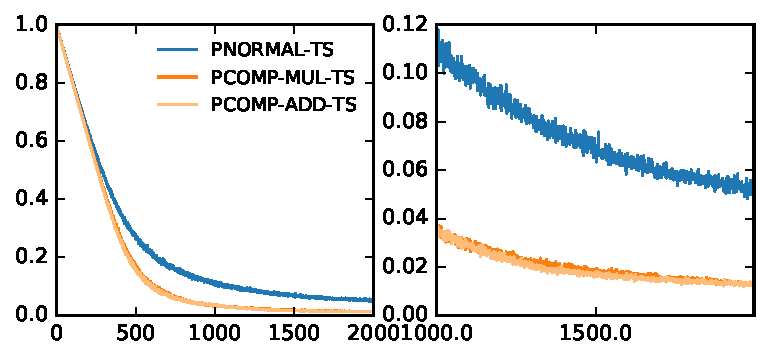
\includegraphics[width=0.9\linewidth]{images/posterior_variance_trace_kinship.pdf}
%	}
%	\subfigure[UMLS]{
%	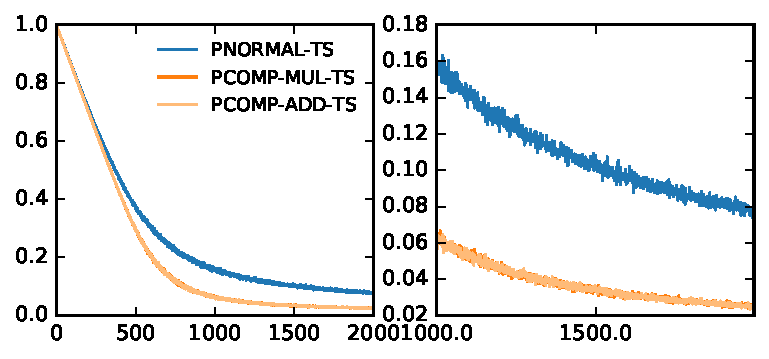
\includegraphics[width=0.9\linewidth]{images/posterior_variance_trace_umls.pdf}
%	}
%	\subfigure[NATION]{
%	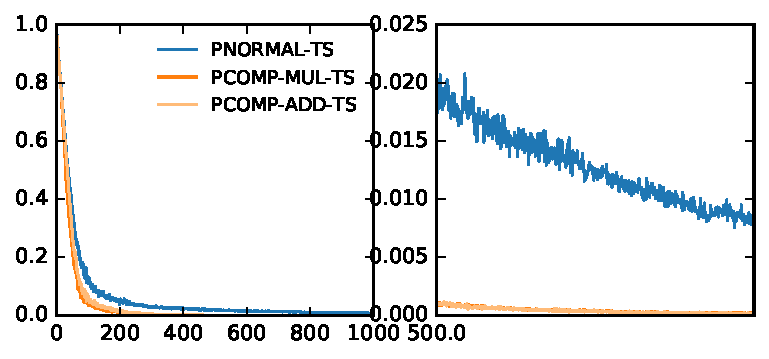
\includegraphics[width=0.9\linewidth]{images/posterior_variance_trace_nation.pdf}
%	}
	
	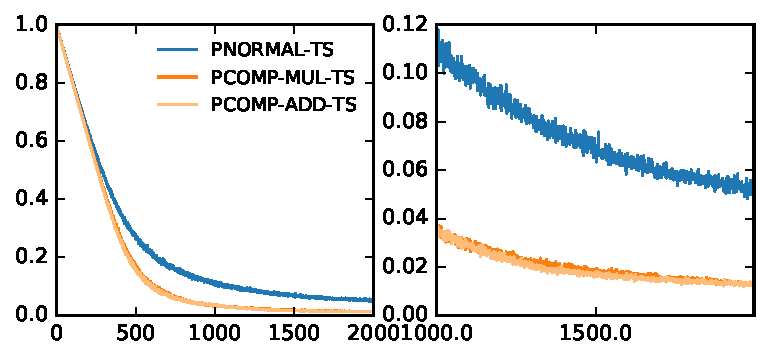
\includegraphics[width=0.9\linewidth]{images/posterior_variance_trace_kinship.pdf}

	\caption{\label{fig:pos_var} Trace plot of mean posterior variance of the non-compositional model and compositional models. Y-axis denotes the average posterior covariance, and X-axis denotes the number of queries. The second plot magnifies the second half of the first plot.}
\end{figure}

We note that the compositional model performs worse than the non-compositional models,
especially than PNORMAL, in this active setting. This is an interesting result because, 
in general, we expect that the model that performs well in the predictive task also shows 
a better performance in the active learning. 
Of course, we also emphasis the difference between two experiments; 
the goal of active acquisition is to maximise the number of triples 
whereas the goal of knowledge completion in Section \ref{sec:exp1} is to maximise 
the predictive performance. Nevertheless, the compositional models do not outperform 
PNORMAL in the active learning.
This result can be partially understood in terms of the balance between 
exploration-exploitation. Figure \ref{fig:pos_var} shows the average posterior variance of 
the entity vectors. We compute the eigenvalues of posterior covariance matrix $\Lambda_i^{-1}$ 
and trace the average eigenvalues over the iterations. 
As shown in the figure, the average variance of the compositional model shrinks much faster 
than the PNORMAL. Because the exploration-exploitation of the Thompson sampling depends on the
posterior uncertainty, the fast shrinkage in the posterior variance may indicate the under 
exploration of the model. One new triple with the compositional models induces multiple new 
observations in the compositional triples, therefore the uncertainties of entities and 
relations are measured less than those with non-compositional model. The most of active 
learning algorithm utilise an uncertainty of a model, and therefore, a model with augmented 
structures such as the relation compositions should be considered more carefully to correctly 
reflect its uncertainty.

\eat{If the samples of the compositional model follows the posterior 
distribution, it may show the similar performance with the passive learning 
scenario, but this assumption does not always hold since the active sampling
path does not correspond to the passive scenario. } %%LX: this looks like too much detail
\eat{
One possible explanation is 
that the naive particle Thompson sampling may not capture the posterior of the 
complex compositional structure, so the particle degenerates over time. Recent
 advances in sequential Monte Carlo may help to solve the problem\cite{gu2015neural,naesseth2014sequential,lindsten2014divide}. 
We leave this for future work.
}
